\section{Introdução}
Citação \cite{Ramadge1989}
\subsection{Sistemas a Eventos Discretos}
\subsection{Controle Supervisório}
\subsection{Controle Modular}
%\subsection{Distinguidores e Variaveis}

\subsection{Processo industrial de manufatura}
A Fig. \ref{fig:processo} apresenta uma simulação para a planta industrial.
A composição da planta é a seguinte:
\begin{itemize}
    \item Mesa centralizadora com teste de chapa;
    \item 5 robôs manipuladores;
    \item 4 prensas;
    \item Esteira para destinação final das peças;
\end{itemize}

TODO: descrever processo de manufatura, aqui ou na introdução?

\begin{figure}[H]%
    \centering
    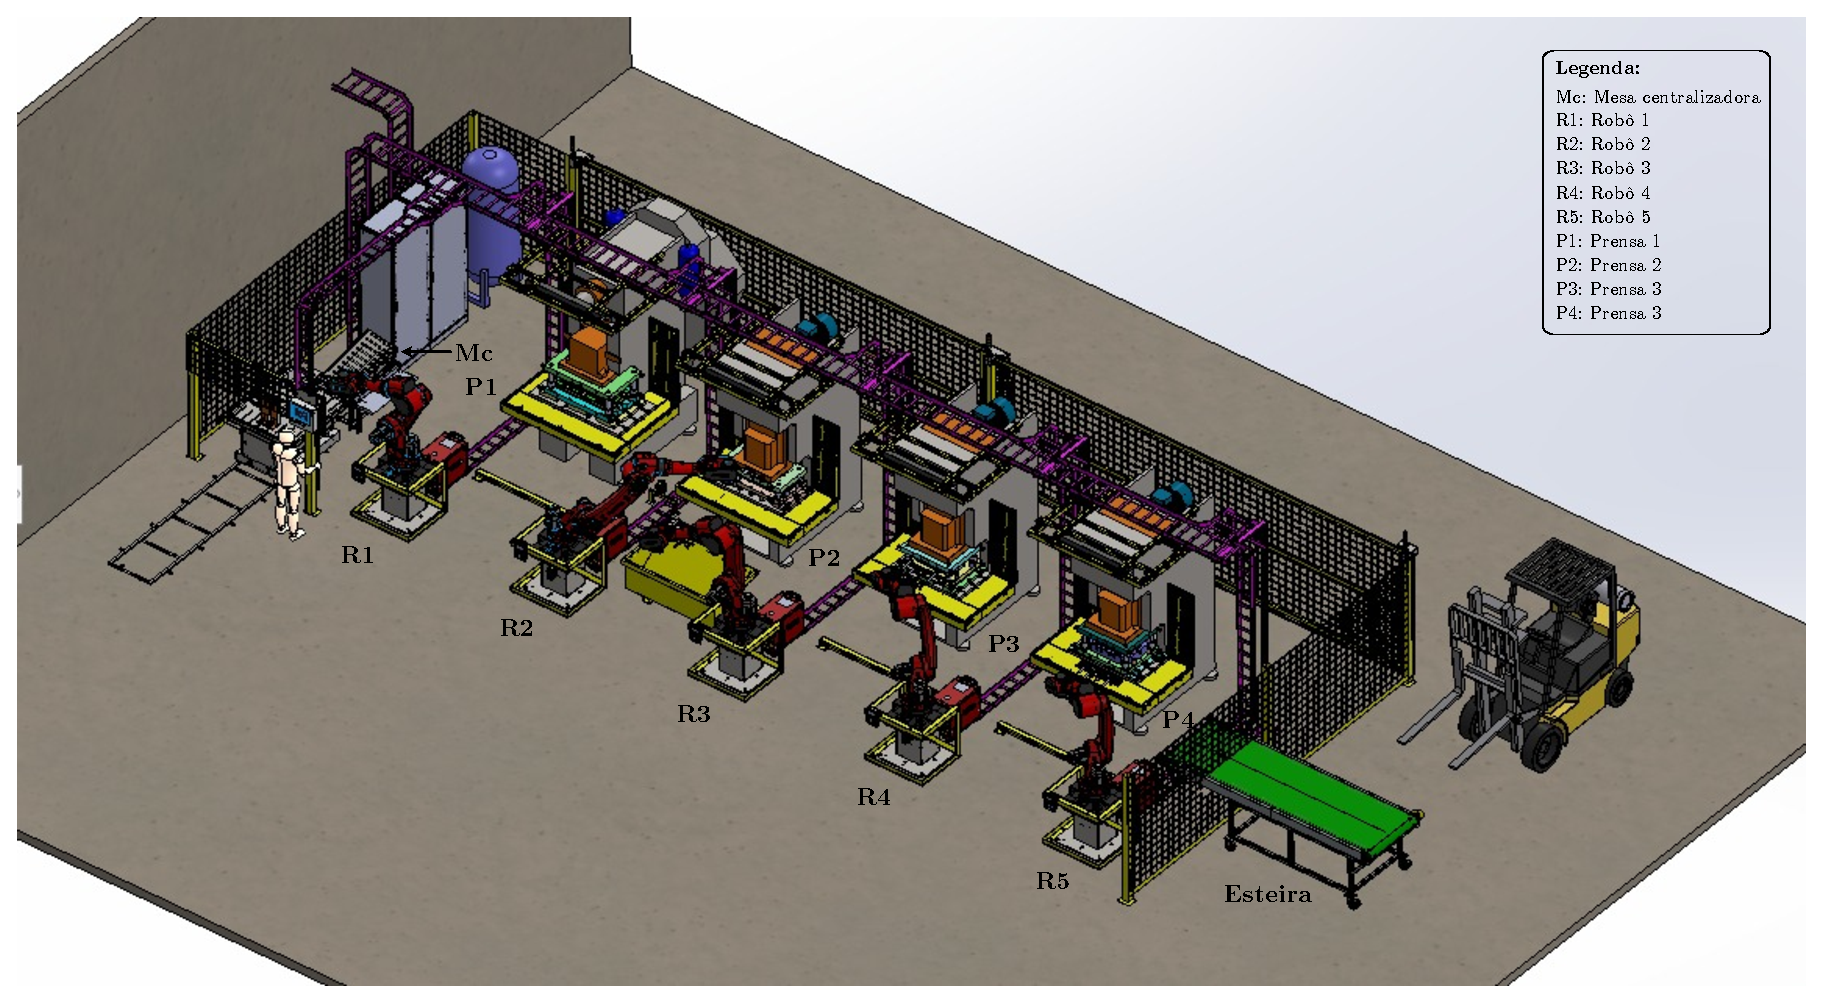
\includegraphics[width=0.8\textwidth]{imagens/processo.eps}
    \caption{Planta industrial}\label{fig:processo}
\end{figure}